\documentclass{report}
\usepackage{graphicx}

\begin{document}

\title{Thesis Proposal}
\author{Adam Yedidia}

\maketitle

\begin{abstract}
% TODO update this!

For my thesis, I propose to write a general-purpose compiler from a programming language of my design to a single-tape, two-symbol Turing machine with as few states as possible. Once this is complete, I propose to write a program in my language that will verify the consistency of Zermelo-Fraenkel set theory (or ZFC), and compile that program down into a Turing machine description. In so doing, I will have created a description for a Turing machine whose behavior cannot be predicted by ZFC. This is true by inspection, because since a logic system cannot prove its own consistency, a logic system cannot prove whether or not a Turing machine that verifies its consistency accepts or rejects.
\end{abstract}

\section{Introduction}
My thesis is split into two chapters. The first chapter relates to the concept of what was done: the substance and importance of what was proven, background on Zermelo-Fraenkel set theory and the Busy Beaver sequence, the exact definition of the Turing machine 

The work of my thesis would not have been possible without first splitting it into two parts: the construction of the compiler, and the 

%%%%%%%%%%%%%%%%%%%%%%%%%%%%
%%%%%% TODO %%%%%%%%%%
%%%%%%%%%%%%%%%%%%%%%%%

\chapter{Concept}

\chapter{Implementation}

The compiler used and referenced in this paper has as its goal to convert a program written in TMD into a description of Turing machine running on a single tape and using a 2-symbol alphabet. In between, the code is passed through two intermediate stages: a description of a Turing machine running on multiple tapes using a 3-symbol alphabet, and a description of a Turing machine running on a single tape using a 4-symbol alphabet. A detailed diagram illustrating this process is visible in Figure~\ref{fig:process}. \\

In this chapter, each of the four representations will be described in turn, from highest- to lowest-level. Additionally, detailed explanations will be given for how the conversion of one representation to the one immediately below it is done.

\begin{figure} 
\begin{center} 
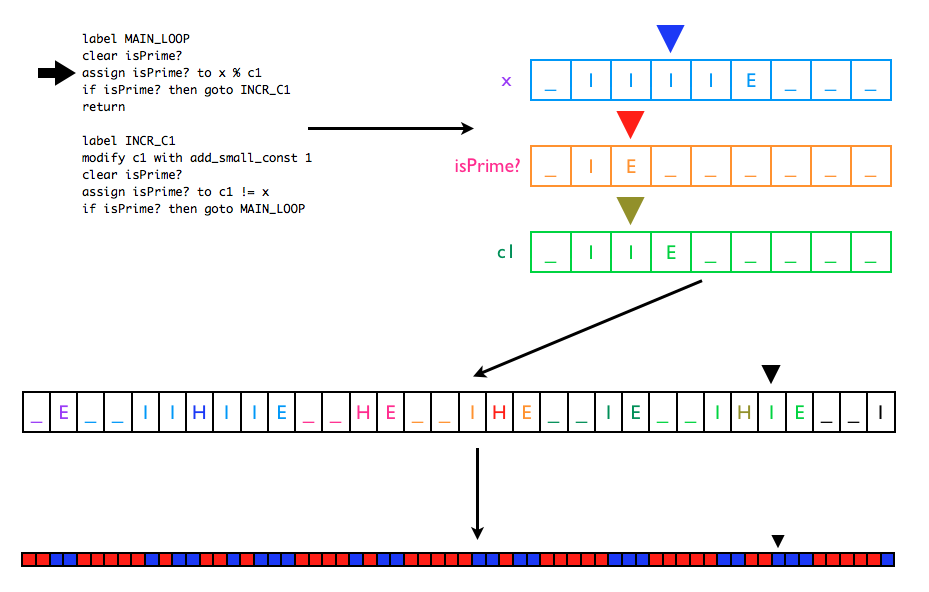
\includegraphics[height=3.25in,width=5in,angle=0]{figs/process.png} 
\caption{This diagram illustrates each of the steps in the conversion between a program written in TMD and a description of a single-tape Turing machine with a binary tape alphabet.\label{fig:process}} 
\end{center} 
\end{figure}  

\section{TMD}

The top-level representation is a program written in the TMD language, which is a language created and designed explicitly for use in this project. TMD is altogether not unlike Assembly Language, although it is more powerful in some ways and weaker in others. \\

There are two types of TMD files. The first type of TMD file is a TMD \emph{main file}. A main file is a file that can be run on its own, but cannot be called by another program. The second type of TMD file is a \emph{function file}. A function file can be called by another program, but cannot be run on its own. The two types of files obey differing syntax, and the differences between them will be explained in further detail in this section.

A TMD program is a sequence of commands. Commands are separated by newlines. Each command is given its own line. \\

\subsection{List of Commands}

The following is a list of possible commands. Let \texttt{x}, \texttt{x1}, \texttt{x2}, and \texttt{x3} be the names of distinct variables, let \texttt{c} be a numerical constant, and let \texttt{f} be the name of a function. Let \texttt{L} be the name of a code label. \\

\textbf{Main files only} \\ \\
\texttt{var x}: Declares a variable with the name \texttt{x}. \\ \\
\texttt{vars x1 x2} \dots: Declares several variables with the names \texttt{x1}, \texttt{x2}, \dots \\

\textbf{Function files only} \\ \\
\texttt{input x1 x2} \dots: Defines the arguments to the function file to be \texttt{x1}, \texttt{x2}, \dots \\ \\\
\texttt{return}: Exits the function and returns to executing wherever the function was called. \\

\textbf{Either file} \\ \\
\texttt{assign x1 to x2} [operation] \texttt{x3}: Changes the value of the variable \texttt{x1} to the result of \texttt{x2} [operation] \texttt{x3}. \\ \\
\texttt{assign x1 to x2} [operation]: Changes the value of the variable \texttt{x1} to the result of the operation [operation] applied to \texttt{x2}. \\ \\
\texttt{modify x1 with} [operation] \texttt{x2}: Changes the value of the variable \texttt{x1} to the result of \texttt{x1} [operation] \texttt{x2}. \\ \\
\texttt{modify x with} [operation] \texttt{c}: Changes the value of the variable \texttt{x} to the result of \texttt{x1} [operation] \texttt{x2}. \\ \\
\texttt{clear x}: Changes the value of the variable \texttt{x} to 0. \\ \\
\texttt{label L}: Declares a label L. \\ \\
\texttt{goto L}: Changes the line of code being executed to the line of code that contains ``\texttt{label L}.'' \\ \\
\texttt{if x goto L}: If the current value of \texttt{x} is a positive integer, then changes the line of code being executed to the line of code that contains ``\texttt{label L}.'' \\ \\
\texttt{function f x1 x2} \dots: Calls the function \texttt{f} with the arguments \texttt{x1}, \texttt{x2}, \dots \\ \\ 
\texttt{accept}: The Turing machine accepts. \\ \\ 
\texttt{reject}: The Turing machine rejects. 

\subsection{Main Files}

Main files contain the body of a program, and can be run. Running a main file will cause the sequence of commands in that main file to be run, starting at the top of the main file. \\

Any variable declared at any point in a main file will be initialized before the execution of the program, with an initial value of 0. As part of their execution, main files can call function files, but they cannot call other main files. \\

Main files may not reach the end of the program without accepting or rejecting. 

\begin{figure} 
\begin{center} 
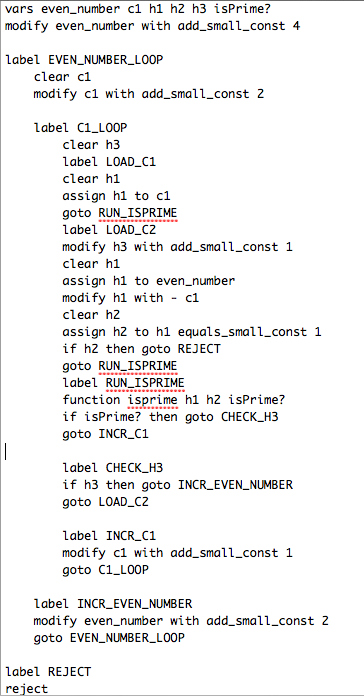
\includegraphics[scale=0.75]{figs/goldbach.png} 
\caption{This is the TMD code for a parsimonious program that will loop if Goldbach's conjecture is true, and reject if it is false. It is provided as an example of a TMD main file. See Figure~\ref{fig:isprime} for the code of the \texttt{isprime} function, which is called by the main body of the program.\label{fig:goldbach}} 
\end{center} 
\end{figure}

\subsection{Function Files}

Function files contain the description of a function. They cannot be run alone; instead, they are called from within a main file or another function file. \\
  
New variables may not be declared from within a function file; instead, any variables needed to perform the computation in the function file are passed in from the file that calls it. Any variables passed into a function file may be modified freely, including integers; that means that there is \emph{no} built-in guarantee that inputs to your function will retain their values after the function runs. \\

Function files may not reach the end of the program without accepting, rejecting, or returning. When a function returns, execution continues at the location of the line beneath where the function was called. Functions never return values; instead, they take effect by modifying the inputs to take on the desired value. \\

Although functions can be called by other functions, they cannot be called recursively (that is, they cannot call themselves and they cannot call functions that eventually call them). This is because the compiler effectively inlines every function when compiling a TMD program to a Turing machine description; no description of a function stack is stored on the tape proper, so a recursive function would cause the compiler to enter an infinite loop. \\

\begin{figure} 
\begin{center} 
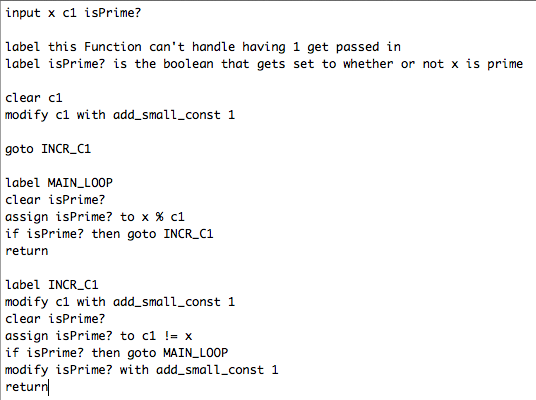
\includegraphics[scale=0.75]{figs/isprime.png} 
\caption{This is the TMD code for a function that will set the value of the input \texttt{isPrime?} to 0 if the input \texttt{x} is not a prime number, and will set the value of \texttt{isPrime?} to a positive integer if \texttt{x} is a prime number. The value of \texttt{x} is not modified by the isprime function, but the value of variable \texttt{c1} may be changed to something arbitrary and the value of \texttt{isPrime?} will be changed to depend on the primality of \texttt{x}. The function's result will depend exclusively on the initial value of \texttt{x}. \label{fig:isprime}} 
\end{center} 
\end{figure}

\end{document}

